
 \begin{figure}
 \centering
 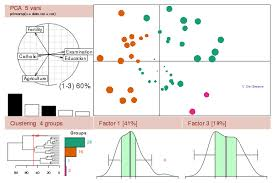
\includegraphics[width=0.97\linewidth]{CRAN}
 \caption{Comprehensive R Archive Network}
 
 \end{figure}
 
  
 %=================================================================== %
 
{R Packages}
 
 
 *  ``10 R packages I wish I knew about earlier" - Drew Conway (Yhat.com, February 2013)
 \bigskip *  ``The HadleyVerse" - Hadley Wickham
 
 
 *   ggplot2, dplyr, reshape, lubridate, stringr
 
 *   With Romain Francois, Dianne Cook and Garret Grolemund.

 \bigskip
 *  Dr Brendan Haplin (UL): lme4 ,TraMineR, Gelman's arm, MASS, foreign. 
 \bigskip
 *  Shiny - Web Applications with \texttt{R}

 
 %=================================================================== %
 
{R Packages}
 
 
 
 
 Some examples of packages are Actuar, written for actuarial science, and
 QRMlib, which complements the Quantitative Risk Management The command library()
 lists all the available packages. 
 
 To load a particular package, for example MASS, we would
 write
 library(MASS)
 
 
 %=================================================================== %
 
 
{Packages}
 
 *  The CRAN package repository features 6107 available packages. 
 *  Packages contain
 various functions and data sets for numerous purposes, e.g.
 \textbf{\textit{ggplot2}} package, \textbf{\textit{AER}} package, \textbf{\textit{survival}} package, etc.
 *  Some packages are part of the basic installation. Others can be
 downloaded from CRAN.
 *  To access all of the functions and data sets in a particular package,
 it must be loaded into the workspace. 
 *  For example, to load the
 \textbf{\textit{ggplot2}} package:

 \begin{framed}
 \begin{verbatim}
 install.packages(ggplot2)
 library(ggplot2)
 \end{verbatim}
 \end{framed}
 
 %==============================================================================================%
 
{4.2 Using and Installing packages}
 
 *  Many packages come with R. To use them in an R session, you need to load the package, as
 previously demonstrated.
 *  Some packages are not automatically installed when you install R but they need to be downloaded
 and installed individually. 
 *  We must first install them using the install.packages()
 function, which typically downloads the package from CRAN and installs it for use. (follow the
 instructions as indicated).

 
 %==============================================================================================%
 
 \begin{framed}
 \begin{verbatim}
 install.packages("ggplot2")
 install.packages("qcc")
 install.packages("sqldf")
 install.packages("RMongo")
 install.packages("randomforest")
 \end{verbatim}
 \end{framed}
 
 
 %==============================================================================================%
 
{4.2.1 Version of R}
 Many packages will require you to have the most recent version of R and also other packages.
 It is a good idea to update regularly.
 
 %==============================================================================================%
 
